\chapter{4541 seriële buscontroller}

\newcolumntype{Y}[1]{%
  >{\small\raggedright\everypar{\hangindent=1em}\arraybackslash}p{#1}%
}

\section{Overzicht}

De 4541 is een buscontroller die compatibel is met de seriële randapparatuurbus van Commodore{\texttrademark} en die de inspanning die nodig is om met apparaten op deze bus te communiceren sterk vermindert.

\section{Mogelijkheden van de 4541}

\subsection{Ondersteuning van versnelde seriële protocolvarianten}

De 4541 ondersteunt de JiffyDOS{\texttrademark}-uitbreidingen op dit protocol, waarmee gegevensoverdrachten ongeveer 10$\times$ sneller verlopen dan met het oorspronkelijke protocol. Van een toekomstige revisie van de 4541 wordt verwacht dat deze het snelle seriële protocol van Commodore ondersteunt, dat in de schijfstations 1571 en 1581 aanwezig is.

\subsection{Processorontlasting via interruptondersteuning}

De 4541 voert seriële communicatie uit onafhankelijk van de microprocessor. Samen met een IRQ-functionaliteit stelt dit software in staat om door te gaan met andere taken terwijl seriële communicatie met randapparaten plaatsvindt, waarbij slechts een korte onderbreking nodig is wanneer het volgende gebeurtenis op de seriële randapparatuurbus optreedt.

\subsection{Onafhankelijkheid van processorsnelheid}

Een groot voordeel van de 4541 is dat deze ook alle tijdsvereisten van communicatie op deze bus afhandelt, waardoor de bus kan worden aangestuurd door een processor die op verschillende snelheden kan werken, zonder de software van de buscontroller aan te hoeven passen.

\subsection{Coëxistentie via open-collectorlogica}

Omdat de 4541 open-collectorlogica gebruikt, kan deze parallel worden gebruikt met bestaande softwarematige implementaties van het busprotocol, waarmee compatibiliteit met bestaande software wordt gewaarborgd. In de MEGA65 is de 4541 in deze configuratie geïnstalleerd, waardoor de bestaande softwarematige communicatiesoftware voor de seriële randapparatuurbus ongewijzigd kan blijven werken.

\section{Werkingsprincipe}

De 4541 biedt een eenvoudige interface: u geeft opdrachten, wacht op een reactie en haalt vervolgens de gegevens op die de opdracht heeft verzameld. Sommige opdrachten vereisen ook een gegevensbyte, die via een apart register wordt aangeboden. Er is ook een register met apparaatinformatie, waarmee u kunt zien wat de 4541 van de huidige status van het meest recent gevraagde apparaat vindt, waaronder of het aanwezig is en of het een van beide of beide uitbreidingen van het JiffyDOS{\texttrademark}- of Commodore{\texttrademark} 128-protocol ondersteunt.

Om bijvoorbeeld de Attention-lijn vrij te geven, schrijft u de juiste commandobyte-waarde (65 = \$41) naar het commandoregister op \$D698 en controleert u vervolgens de voltooiingsstatus in het statusregister op \$D697, zoals weergegeven in het volgende voorbeeld in BASIC65:

\begin{screencode}
  10 POKE $D698,$41
  20 IF ( PEEK($D697) AND $20 ) = $00 GOTO 20
  30 PRINT "GEREED"
\end{screencode}

De 4541 implementeert een reeks opdrachten die nauw aansluiten bij de KERNAL-aanroepen die worden gebruikt om de IEC-bus op de C64 en verwante computers te besturen. In de meeste gevallen is er één bijbehorende opdracht voor de 4541, hoewel u in een aantal gevallen twee opdrachten moet geven, zoals samengevat in de volgende tabel:

\index{IEC-controlleropdrachten}
\begin{center}
    \small{
    \setlength{\def\arraystretch{1.5}\tabcolsep}{6pt}
    \begin{longtable}{|c|L{9cm}|}
        \hline
        \textbf{KERNAL-aanroep} & \textbf{Betekenis en bijbehorende 4541-opdracht(en)}\\
        \hline
        \endhead
        \$FF93 LSTNSA & Verzend het secundaire LISTEN-adres.  \\         & 4541-equivalent: Gegevens = Binair OR van \$60 en het gewenste        secundaire adres.  Opdracht \$30. Vervolgens opdracht \$41 om de        Attention-lijn vrij te geven. \\
        \hline
        \$FF96 TALKSA & Verzend het secundaire TALK-adres.  \\         & 4541-equivalent: Gegevens = Binair OR van \$60 en het gewenste        secundaire adres.  Opdracht \$30. Vervolgens opdracht \$41 om de        Attention-lijn vrij te geven. \\
        \hline
        \$FFA5 IECIN & Ontvang een byte van de seriële randapparatuurbus.  \\         & 4541-equivalent : Opdracht \$32. De ontvangen byte is beschikbaar        in het gegevensregister na voltooiing.  \\
        \hline
        \$FFA8 IECOUT & Verzend een byte naar de seriële randapparatuurbus.  \\         & 4541-equivalent : Gegevens = de te verzenden byte. Opdracht \$31 (of \$30 indien de byte        onder Attention wordt verzonden). \\
        \hline
        \$FFA8 UNTALK  & Verzend UNTALK-opdracht naar de seriële randapparatuurbus.  \\        & 4541-equivalent : Gegevens = \$5F. Opdracht \$30. \\
        \hline
        \$FFAB UNLISTN  & Verzend UNLISTEN-opdracht naar de seriële randapparatuurbus.  \\        & 4541-equivalent : Gegevens = \$3F. Opdracht \$30. \\
        \hline
        \$FFB1 LISTEN  & Verzend het LISTEN-commando naar de seriële randapparatuurbus.  \\        & 4541-equivalent: Gegevens = \$20 plus het apparaatnummer. Opdracht \$30. \\
        \hline
        \$FFB4 TALK  & Verzend het TALK-commando naar de seriële randapparatuurbus.  \\        & 4541-equivalent: Gegevens = \$40 plus het apparaatnummer. Opdracht \$30. \\
        \hline
        \$FFB7 READSS & Lees de status van de seriële randapparatuurbus.  \\        & 4541-equivalent: Lees de statusbits vanaf \$D698. Voor        het gemak hebben de        bovenste bits van deze statusbyte dezelfde indeling als in        de KERNAL. \\
        \hline
    \end{longtable}
    }
\end{center}

De 4541 is zeer gehoorzaam: vraagt u hem iets nieuws, dan begint hij daar onmiddellijk mee, zelfs midden in een andere taak -- zelfs al is hij halverwege het verzenden van een byte gegevens naar de seriële randapparatuurbus!

U dient dan ook altijd te wachten totdat de IRQREADY-bit in \$D697 is gezet voordat u een commando geeft of de statusbits leest, zodat u er zeker van bent dat de controller de laatste gevraagde taak heeft afgerond.

\section{Voorbeelden}

\subsection{De status van het DOS-kanaal lezen}

Het volgende BASIC65-programma kan worden gebruikt om met een apparaat op de seriële randapparatuurbus te communiceren. Omdat het de 4541 gebruikt en niet de CBDOS van de C65/MEGA65, negeert dit programma het interne 3.5''-schijfstation, omdat dat station niet op de seriële randapparatuurbus is aangesloten.

\begin{screencode}
10 REM BREEK EEN EVENTUEEL LOPEND 4541-COMMANDO af
20 POKE $D698,$00
30 REM RESET DE SERIELE RANDAPPARATUURBUS DOOR
40 REM DE RESETPIN 1 SECOND LANG LAAG TE HOUDEN
50 POKE $D698,$72 : SLEEP 1 : POKE $D698,$52
60 REM GUN AANGESLOTEN APPARATEN NA RESET TIJD OM GEREED TE KOMEN
70 SLEEP 2: REM HET DUURT EVEN VOOR DE 1541 GERESET IS!
80 REM SELECTEER HET APPARAATNUMMER WAARNAAR GELUISTERD WORDT
90 D = 8
100 PRINT"DEVICE"; D; "TALK"
110 POKE $D699,$40 + D : POKE $D698,$30 : GOSUB 1000
120 PRINT "SECUNDAIR ADDRES 15"
130 POKE $D699,$6F : POKE $D698,$30 : GOSUB 1000
140 PRINT"OMKEREREN NAAR LUISTEREN"
150 POKE $D698,$35 : GOSUB 1000
160 PRINT "LEES DOSSTATUS"
170 POKE $D698,$32 : GOSUB 1000
180 PRINT CHR$( PEEK($D699) );
190 CC = CC + 1 : IF CC < 200 GOTO 180
999 END
1000 REM WACHT TOT DE 4541 HET COMMANDO HEEFT AFGEROND
1010 S=PEEK($D697) : IF (S AND 32) = 32 GOTO 1020
1020 GOTO 1000
1030 IF S AND 128 THEN PRINT "DEVICE NIET AANWEZIG" : END
1040 RETURN
\end{screencode}

Als u een 1581 met een JiffyDOS{\texttrademark}-ROM heeft aangesloten, toont dit programma bij uitvoering het volgende:

\begin{screencode}
READY.
RUN
DEVICE 8 TALK
SECUNDAIR ADRES 15
OMKEREN NAAR LUISTEREN
LEES DOSSTATUS
73,(C) 1989 JIFFYDOS 6.0 1581,00,00
00, OK,00,00
00, OK,00,00
00, OK,00,00
...
00, OK,0
READY.
\end{screencode}

\section{Commandoreferentie}

De volgende tabel geeft een overzicht van de door de 4541 ondersteunde commandocodes.

\begin{center}
    \setlength{\def\arraystretch{1.5}\tabcolsep}{6pt}
    \begin{longtable}{|c|L{8cm}|}
        \hline
        \textbf{Commandobyte} & \textbf{Actie} \\
        \hline
        \endhead
        \multicolumn{2}{c}{\textbf{Lopende commando's onderbreken}} \\
        \hline
        \$00 & Onderbreek elk uitgevoerd commando. \\
        \hline
        \$01 & Herstel de toestand van de controller: ATN, CLK, DATA en SRQ loslaten en de standaard protocolselectie inschakelen. \\
        \hline
        \multicolumn{2}{c}{\textbf{Bit-bashing-commando's}} \\
        \hline
        \$41 & Attention-lijn (ATN) loslaten naar 5V. \\
        \hline
        \$61 & Attention-lijn (ATN) naar 0V trekken. \\
        \hline
        \$43 & Kloklijn (CLK) loslaten naar 5V. \\
        \hline
        \$63 & Kloklijn (CLK) naar 0V trekken. \\
        \hline
        \$44 & Gegevenslijn (DATA) loslaten naar 5V. \\
        \hline
        \$64 & Gegevenslijn (DATA) naar 0V trekken. \\
        \hline
        \$53 & Snelle seriële kloklijn (SRQ) loslaten naar 5V. \\
        \hline
        \$73 & Snelle seriële kloklijn (SRQ) naar 0V trekken. \\
        \hline
\$52 & Laat de resetlijn (RESET) los op 5V. \\
        \hline
\$72 & Trek de resetlijn (RESET) naar 0V. \\
        \hline
\$4C & Laat alle lijnen (ATN, CLK, DATA, SRQ, RESET) los op 5V. \\
        \hline
\multicolumn{2}{c}{\textbf{Protocolvariant-besturingscommando's}} \\
        \hline
\$4A & Sta het aanvragen van de JiffyDOS{\texttrademark}        uitbreiding voor het seriële protocol toe. \\
        \hline
\$6A & Sta het aanvragen van de JiffyDOS{\texttrademark}        uitbreiding voor het seriële protocol niet toe. \\
        \hline
\$46 & Sta het aanvragen van de Commodore{\texttrademark} 1571/1581        snelle seriële uitbreiding voor het seriële protocol toe. \\
        \hline
\$66 & Sta het aanvragen van de Commodore{\texttrademark} 1571/1581        snelle seriële uitbreiding voor het seriële protocol niet toe. \\
        \hline
\$50 & Sta het aanvragen van alle seriële uitbreidingen toe. \\
        \hline
\$70 & Sta het aanvragen van alle seriële uitbreidingen niet toe. \\
        \hline

\multicolumn{2}{c}{\textbf{Seriële busprotocolcommando's}} \\
        \hline
\$30 & Verzend een byte in \$D699 onder Attention. De Attention-lijn        wordt aan het einde van de transactie op 0V gehouden. \\
        \hline
\$31 & Verzend een byte in \$D699 zonder Attention. De Attention-lijn        wordt losgelaten indien deze voorafgaand was geactiveerd. \\
        \hline
\$32 & Ontvang een byte van de seriële randapparatuurbus. Er moet een        vooraf geactiveerde spreker (``\textbf{talk}er'') aanwezig zijn. De ontvangen byte wordt        opgeslagen in \$D699. \\
        \hline
\$33 & GERESERVEERD \\
        \hline
\$34 & Verzend een byte en geef einde-aanduiding (EOI) aan. De Attention-lijn wordt voorafgaand        aan de verzending losgelaten indien deze was geactiveerd. \\
        \hline
\$35 & Draai om van spreker (``\textbf{talk}er'') naar luisteraar (``\textbf{listen}er''). \\
        \hline

\multicolumn{2}{c}{\textbf{Commando's voor de protocoltiming}} \\
        \hline
        \$80 & Reset de protocoltiming naar de standaardwaarden. \\ \hline        \$81 & Stel de T\textsubscript{R}-vertraging in (1 -- 255 microseconden). De oude waarde kan        worden gelezen uit \$D699.\\ \hline        \$82 & Stel de T\textsubscript{TK}-vertraging in (1 -- 255 microseconden). De oude waarde kan        worden gelezen uit \$D699.\\ \hline        \$83 & Stel de T\textsubscript{DC}-time-out in (1 -- 255 milliseconden). De oude waarde kan        worden gelezen uit \$D699.\\ \hline        \$84 & Stel de T\textsubscript{BB}-vertraging in (1 -- 255 microseconden). De oude waarde kan        worden gelezen uit \$D699.\\ \hline        \$85 & Stel de T\textsubscript{HA}-vertraging in (1 -- 255 microseconden). De oude waarde kan        worden gelezen uit \$D699.\\ \hline        \$86 & Stel de T\textsubscript{ST}-vertraging in (1 -- 255 microseconden). De oude waarde kan        worden gelezen uit \$D699.\\ \hline        \$87 & Stel de T\textsubscript{VT}-vertraging in (1 -- 255 microseconden). De oude waarde kan        worden gelezen uit \$D699.\\ \hline        \$88 & Stel de T\textsubscript{AL}-vertraging in (1 -- 255 microseconden). De oude waarde kan        worden gelezen uit \$D699.\\ \hline        \$89 & Stel de T\textsubscript{AC}-vertraging in (1 -- 255 microseconden). De oude waarde kan        worden gelezen uit \$D699.\\ \hline        \$8A & Stel de T\textsubscript{AT}-vertraging in (1 -- 255 milliseconden). De oude waarde kan        worden gelezen uit \$D699.\\ \hline        \$8B & Stel de T\textsubscript{H}-vertraging in (1 -- 255 milliseconden). De oude waarde kan        worden gelezen uit \$D699. {\em Deze waarde heeft momenteel geen effect, omdat de 4541 een werkelijk oneindige wachttijd door een luisteraar mogelijk maakt, met uitzondering van bytes die onder Attention worden verzonden, waarbij in plaats daarvan T\textsubscript{HA} wordt gebruikt.}\\ \hline        \$8C & Stel de T\textsubscript{NE}-vertraging in (1 -- 255 microseconden). De oude waarde kan        worden gelezen uit \$D699.\\ \hline        \$8D & Stel de T\textsubscript{F}-vertraging in (4 -- 1020 microseconden). De oude waarde kan        worden gelezen uit \$D699, geschaald met een factor 4.\\ \hline        \$8E & Stel de T\textsubscript{YE}-vertraging in (1 -- 255 microseconden). De oude waarde kan        worden gelezen uit \$D699.\\ \hline        \$8F & Stel de T\textsubscript{EI}-vertraging in (1 -- 255 microseconden). De oude waarde kan        worden gelezen uit \$D699.\\ \hline        \$90 & Stel de T\textsubscript{AR}-vertraging in (1 -- 255 microseconden). De oude waarde kan        worden gelezen uit \$D699.\\ \hline        \$91 & Stel de T\textsubscript{JT}-vertraging in (4 -- 1020 microseconden). De oude waarde kan        worden gelezen uit \$D699, geschaald met een factor 4.\\ \hline        \$92 & Stel de T\textsubscript{J0}-vertraging in (1 -- 255 microseconden). De oude waarde kan        worden gelezen uit \$D699.\\ \hline        \$93 & Stel de T\textsubscript{J1}-vertraging in (1 -- 255 microseconden). De oude waarde kan        worden gelezen uit \$D699.\\ \hline        \$94 & Stel de T\textsubscript{J2}-vertraging in (1 -- 255 microseconden). De oude waarde kan        worden gelezen uit \$D699.\\ \hline        \$95 & Stel de T\textsubscript{J3}-vertraging in (1 -- 255 microseconden). De oude waarde kan        worden gelezen uit \$D699.\\ \hline        \$96 & Stel de T\textsubscript{J4}-vertraging in (1 -- 255 microseconden). De oude waarde kan        worden gelezen uit \$D699.\\ \hline        \$97 & Stel de T\textsubscript{J5}-vertraging in (1 -- 255 microseconden). De oude waarde kan        worden gelezen uit \$D699.\\ \hline        \$98 & Stel de T\textsubscript{J6}-vertraging in (1 -- 255 microseconden). De oude waarde kan        worden gelezen uit \$D699.\\ \hline        \$99 & Stel de T\textsubscript{J7}-vertraging in (1 -- 255 microseconden). De oude waarde kan        worden gelezen uit \$D699.\\ \hline        \$9A & Stel de T\textsubscript{J8}-vertraging in (1 -- 255 microseconden). De oude waarde kan        worden gelezen uit \$D699.\\ \hline        \$9B & Stel de T\textsubscript{J9}-vertraging in (1 -- 255 microseconden). De oude waarde kan        worden gelezen uit \$D699.\\ \hline        \$9C & Stel de T\textsubscript{J10}-vertraging in (1 -- 255 microseconden). De oude waarde kan        worden gelezen uit \$D699.\\ \hline        \$9D & Stel de T\textsubscript{J11}-vertraging in (1 -- 255 microseconden). De oude waarde kan        worden gelezen uit \$D699.\\ \hline        \$9E & Stel de T\textsubscript{JR}-vertraging in (1 -- 255 microseconden). De oude waarde kan        worden gelezen uit \$D699.\\ \hline        \$9F & Stel de T\textsubscript{FS}-vertraging in (1 -- 255 microseconden). De oude waarde kan        worden gelezen uit \$D699.\\ \hline        \$A0 & Stel de T\textsubscript{FF}-vertraging in (1 -- 255 microseconden). De oude waarde kan        worden gelezen uit \$D699.\\ \hline        \$A1 & Stel de T\textsubscript{PULLUP}-vertraging in (1 -- 255 microseconden). De oude waarde kan        worden gelezen uit \$D699.\\ \hline        \$A2 & Stel de T\textsubscript{JD}-vertraging in (4 -- 1020 microseconden). De oude waarde kan        worden gelezen uit \$D699, geschaald met een factor 4.\\ \hline        \$A3 & Stel de T\textsubscript{J12}-vertraging in (1 -- 255 microseconden). De oude waarde kan        worden gelezen uit \$D699.\\ \hline                \multicolumn{2}{c}{\textbf{Diagnostische opdrachten}} \\
        \hline
\$D0 & Activeer de optionele geïntegreerde datalogger indien        ingeschakeld. \\
        \hline
\$D1 & Begin met het uitzenden van een 1 kHz-pulstrein op de CLK- en        DATA-lijnen. Dit duurt voort totdat een ander commando het        onderbreekt. \\
        \hline
    \end{longtable}
\end{center}


\section{Registertabel}

De 4541 heeft de volgende registers:

\setlength{\tabcolsep}{0pt}
\begin{longtable}{|C{12.5mm}|C{12.5mm}|C{12.5mm}|C{12.5mm}|C{12.5mm}|C{12.5mm}|C{12.5mm}|C{12.5mm}|C{12.5mm}|C{12.5mm}|}
\hline
{\bf{HEX}} & {\bf{DEC}} & {\bf{DB7}} & {\bf{DB6}} & {\bf{DB5}} & {\bf{DB4}} & {\bf{DB3}} & {\bf{DB2}} & {\bf{DB1}} & {\bf{DB0}} \\
\hline
\endfirsthead
\multicolumn{3}{l@{}}{\ldots vervolgd}\\
\hline
{\bf{HEX}} & {\bf{DEC}} & {\bf{DB7}} & {\bf{DB6}} & {\bf{DB5}} & {\bf{DB4}} & {\bf{DB3}} & {\bf{DB2}} & {\bf{DB1}} & {\bf{DB0}} \\
\endhead
\multicolumn{3}{l@{}}{vervolgd \ldots}\\
\endfoot
\hline
\endlastfoot
\footnotesize  D694\index{Registers!\$D694} \index{Registers!54932} & \footnotesize 54932 & \multicolumn{8}{c|}{\footnotesize DATALOG0\index{Registers!DATALOG0}}\\
\hline
\footnotesize  D695\index{Registers!\$D695} \index{Registers!54933} & \footnotesize 54933 & \multicolumn{8}{c|}{\footnotesize DATALOG1\index{Registers!DATALOG1}}\\
\hline
\footnotesize  D697\index{Registers!\$D697} \index{Registers!54935} & \footnotesize 54935 & \footnotesize IRQFLAG & \footnotesize IRQRX & \footnotesize IRQRDY & \footnotesize IRQTO & \footnotesize IRQEN & \footnotesize IRQRXEN & \footnotesize IRQRDYEN & \footnotesize IRQTOEN \\
\hline
\footnotesize  D698\index{Registers!\$D698} \index{Registers!54936} & \footnotesize 54936 & \footnotesize STNODEV & \footnotesize STNOEOI & \footnotesize STSRQ & \footnotesize STVERIFY & \footnotesize STC & \footnotesize STD & \footnotesize STTO & \footnotesize STDDIR \\
\hline
\footnotesize  D699\index{Registers!\$D699} \index{Registers!54937} & \footnotesize 54937 & \multicolumn{8}{c|}{\footnotesize DATA\index{Registers!DATA}}\\
\hline
\footnotesize  D69A\index{Registers!\$D69A} \index{Registers!54938} & \footnotesize 54938 & \footnotesize PRESENT & \multicolumn{2}{c|}{\footnotesize PROT\index{Registers!PROT}}& \footnotesize DIATN & \multicolumn{4}{c|}{\footnotesize DEVNUM\index{Registers!DEVNUM}}\\
\hline
\end{longtable}
\begin{itemize}
\item{\bf{DATA}\index{Registers!DATA}} De gegevensbyte die van de IEC-bus wordt gelezen
\item{\bf{DATALOG0}\index{Registers!DATALOG0}} Toegang tot de geïntegreerde datalogger in de IEC-controller
\item{\bf{DATALOG1}\index{Registers!DATALOG1}} Toegang tot de geïntegreerde datalogger in de IEC-controller
\item{\bf{DEVNUM}\index{Registers!DEVNUM}} De onderste 4 bits van het op dat moment geselecteerde apparaatnummer
\item{\bf{DIATN}\index{Registers!DIATN}} Het apparaat wordt momenteel in de attention-toestand gehouden
\item{\bf{IRQEN}\index{Registers!IRQEN}} Schakelt de interrupts in indien deze is gezet
\item{\bf{IRQFLAG}\index{Registers!IRQFLAG}} Interruptvlag. Deze wordt gezet indien een IRQ-gebeurtenis wordt geactiveerd.
\item{\bf{IRQRDY}\index{Registers!IRQRDY}} Gezet indien gereed om een opdracht te verwerken
\item{\bf{IRQRDYEN}\index{Registers!IRQRDYEN}} Schakelt de TX-interruptbron in indien deze is gezet
\item{\bf{IRQRX}\index{Registers!IRQRX}} Gezet indien een byte van een luisteraar is ontvangen.
\item{\bf{IRQRXEN}\index{Registers!IRQRXEN}} Schakelt de RX-interruptbron in indien deze is gezet
\item{\bf{IRQTO}\index{Registers!IRQTO}} Gezet indien een protocol-timeout is opgetreden, bijv. wanneer het apparaat niet wordt gevonden.
\item{\bf{IRQTOEN}\index{Registers!IRQTOEN}} Schakelt de timeout-interruptbron in indien deze is gezet
\item{\bf{PRESENT}\index{Registers!PRESENT}} Het apparaat is aanwezig
\item{\bf{PROT}\index{Registers!PROT}} Protocolondersteuning van het apparaat (5=C128/C65 FAST, bit 6 = JiffyDOS(tm))
\item{\bf{STC}\index{Registers!STC}} Toestand van de CLK-lijn
\item{\bf{STD}\index{Registers!STD}} Toestand van de DATA-lijn
\item{\bf{STDDIR}\index{Registers!STDDIR}} De gegevensrichting op het moment dat een timeout optreedt.
\item{\bf{STNODEV}\index{Registers!STNODEV}} Het apparaat is niet aanwezig
\item{\bf{STNOEOI}\index{Registers!STNOEOI}} End of Indicate (EOI/EOF)
\item{\bf{STSRQ}\index{Registers!STSRQ}} Toestand van de SRQ-lijn
\item{\bf{STTO}\index{Registers!STTO}} Er is een timeout opgetreden
\item{\bf{STVERIFY}\index{Registers!STVERIFY}} Er is een verificatiefout opgetreden
\end{itemize}


\section{Seriële bustiming}

Dit hoofdstuk beschrijft de tijdsvereisten voornamelijk vanuit het perspectief van een buscontroller. Indien u seriële busapparaten ontwerpt, besteed dan zorgvuldig aandacht aan de manier waarop deze tijdsvereisten de apparaten beïnvloeden.


\subsection{Een byte onder Attention verzenden}

Wanneer de controller de aandacht van één of meer apparaten op de bus wil trekken, gebruikt hij de ATN-lijn om dit aan te geven: hij trekt deze laag naar 0V en stuurt vervolgens één of meer bytes die door alle apparaten op de bus worden ontvangen.

De SRQ-lijn is niet actief in deze transactie.

Samengevat:

\begin{enumerate}
\item De controller trekt de ATN naar 0V en laat de CLK-, DATA- en SRQ-lijnen los indien hij een van deze op 0V hield.\item Alle apparaten op de bus merken op dat de ATN-lijn op 0V staat en geven dit aan door de DATA-lijn naar 0V te trekken. De controller kan niet zien noch hoeveel apparaten er hebben gereageerd, noch of alle apparaten op de bus hebben gereageerd; hij kan enkel vaststellen dat ten minste één apparaat heeft gereageerd.\item Indien geen enkel apparaat reageert, blijft DATA op 5V, omdat niemand deze naar beneden trekt, en geeft de controller een DEVICE NOT PRESENT-fout aan.\item Terwijl de controller wacht op reactie van de apparaten, trekt hij ook de CLK-lijn naar 0V, doorgaans kort nadat hij de ATN-lijn naar 0V heeft getrokken.\item Nadat de controller enige tijd heeft gewacht, doorgaans 1 milliseconde, neemt hij aan dat alle apparaten die op het ATN-verzoek zullen reageren, dat inmiddels hebben gedaan.\item Vervolgens laat de controller de CLK-lijn los naar 5V om aan te geven dat hij een byte gegevens op de bus wil verzenden. Dit vormt het begin van het verzenden van een byte onder Attention. Al deze voorgaande stappen hadden tot doel de ATN-communicatie tot stand te brengen.\item De controller wacht nu tot alle apparaten hun bereidheid om een byte te ontvangen aangeven door de DATA-lijn terug naar 5V te laten gaan. Omdat de bus open collector is, kan zelfs één enkel apparaat dat nog niet gereed is, de DATA-lijn naar 0V blijven trekken, waardoor de controller moet wachten. Indien dit te lang duurt, kan de controller opgeven en een time-out aangeven.\item Zodra het laatste apparaat heeft aangegeven gereed te zijn om gegevens te ontvangen, wacht de controller nog iets langer om er zeker van te zijn dat alle apparaten hun laatste voorbereidingen voor het ontvangen van een byte kunnen afronden. Dit duurt niet lang.\item Na die wachttijd begint de controller met het verzenden van de 8 bits gegevens, te beginnen met het minst significante bit (LSB), oftewel bit 0. Voor elk bit trekt hij eerst de CLK-lijn laag om aan te geven dat er gegevens op de bus worden geladen, trekt de DATA-lijn naar 0V als hij een 0-bit wenst te verzenden, of laat deze naar 5V zweven als hij een 1-bit wenst te verzenden, en laat vervolgens de CLK-lijn weer los naar 5V en houdt deze daar enige tijd. De timing van dit proces is van kritiek belang: als de CLK te kort laag of hoog is, raken de apparaten in de war en kunnen zij een of meer bits missen, wat op de bus tot volledige chaos leidt.\item Nadat de controller het laatste bit heeft verzonden, houdt hij de CLK-lijn laag en laat de DATA-lijn los. Hij verwacht dat een of meer apparaten binnen korte tijd de DATA-lijn naar 0V trekken om de ontvangst van de byte te bevestigen. Indien dit niet gebeurt, kan de controller een time-out of een DEVICE NOT PRESENT-fout melden.\item Aan het einde hiervan houdt de controller de CLK-lijn op 0V en houden de apparaten de DATA-lijn op 0V. Deze combinatie dient om elkaar te vertellen dat de controller nog geen volgende byte wenst te verzenden en dat de apparaten nog niet gereed zijn om de volgende byte te ontvangen.\item Indien de controller meer bytes onder Attention wenst te verzenden, herhaalt hij dit proces vanaf de stap waarin hij de CLK-lijn naar 5V liet los.\item Indien het echter de laatste byte betrof die onder deze Attention-aanvraag werd verzonden, wacht de controller een korte tijd en laat vervolgens de ATN-lijn los.
\end{enumerate}

\begin{center}
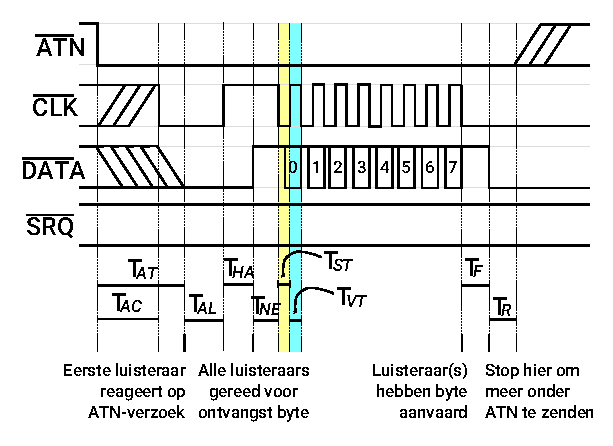
\includegraphics{dutch/images/IEC-Timing-Diagrams/IEC-Timing-Diagram-ATN-Send-Byte}
\end{center}

\begin{center}
    \setlength{\def\arraystretch{1.5}\tabcolsep}{6pt}
    \small {
    \begin{longtable}{|L{0.6cm}|c|c|c|c|L{6cm}|}
      \hline
        \multicolumn{2}{|c|}{\textbf{Symbool}} & \textbf{Min} & \textbf{4541} & \textbf{Max} & \textbf{Omschrijving} \\
        \hline
        \endhead
        \multicolumn{2}{|c|}{T\textsubscript{AT}} & --  & 1000 & $\infty$ &        Reactietijd van het apparaat op Attention. {\em Een apparaat moet          binnen deze tijd op het ATN-verzoek reageren. Indien geen enkel          apparaat binnen deze tijd reageert, volgt een DEVICE NOT PRESENT-fout.          Apparaten dienen derhalve de typische waarde van 1000          microseconden aan te houden.} \\
        \hline
        \multicolumn{2}{|c|}{T\textsubscript{AC}} & --  & 20 & $\infty$? &        Tijd tussen het laag trekken van ATN en het laag trekken van CLK. \\
        \hline
        \multicolumn{2}{|c|}{T\textsubscript{AL}} & --  & 1000 & $\infty$? &        Tijd tussen de reactie van het eerste apparaat op ATN en het loslaten van CLK        door de controller naar 5V. \\
        \hline
        \multicolumn{2}{|c|}{T\textsubscript{HA}} & -- & 64 ms & $\infty$ & Luisteraar-wachttijd. {\em Het protocol staat een luisteraar toe om gedurende een          willekeurige periode of helemaal niet te wachten. De 4541 staat dit niet toe          bij ATN-verzoeken.} \\
        \hline
        \multicolumn{2}{|c|}{T\textsubscript{NE}} & --  & 40 & 200 &        Niet-EOI-tijdskanaalreactie op ``Gereed voor gegevens''. {\em Indien          dit interval te lang is, wordt de byte als een EOI-byte          geïnterpreteerd en zullen de apparaten een EOI-reactie vereisen (zie T\textsubscript{EI}).} \\
        \hline
        \multicolumn{2}{|c|}{T\textsubscript{ST}} & 20*  & 35 & $\infty$ &        Bitinsteltijd. {\em Wordt aangeduid als T\textsubscript{S} in          de C64 Programmer's Reference Guide.}\\
        \hline
        \multicolumn{2}{|c|}{T\textsubscript{VT}} & 20*  & 35 & $\infty$ &        Bitgeldigheid vasthoudtijd. {\em Wordt aangeduid als          T\textsubscript{V} in de C64 Programmer's Reference Guide.} \\
        \hline
        \multicolumn{2}{|c|}{T\textsubscript{F}} & --  & 1000 & 1000 &        Frame-handshake (bevestiging) time-out. \\
        \hline
        \multicolumn{2}{|c|}{T\textsubscript{R}} & 20  & 200 & $\infty$ &        Tijd tussen het ontvangen van de framebevestiging en        het loslaten van de ATN-lijn naar 5V. \\
        \hline
        \multicolumn{6}{l}{\em Alle tijdseenheden zijn uitgedrukt in microseconden, tenzij          anders aangegeven.} \\        \multicolumn{6}{Y{10cm}}{*{}          De Commodore{\texttrademark} 64 Programmer's Reference          Guide stelt dat T\textsubscript{S} en          T\textsubscript{V} elk een minimumduur van 20 microseconden dienen te hebben.          Onze onderzoeken wijzen uit dat bij communicatie met een          1541 veilige waarden voor          T\textsubscript{ST} en T\textsubscript{VT} dichter bij 70          microseconden liggen.
        }
          \\

    \end{longtable}
    }
\end{center}

\subsection{JiffyDOS{\texttrademark}-protocolaanvraag}

Indien ondersteuning voor de JiffyDOS{\texttrademark}-protocoluitbreiding is ingeschakeld, vraagt de 4541 deze slechts aan tijdens de verzending van TALK- en LISTEN-commando's. Dat wil zeggen: wanneer een byte onder Attention wordt gestuurd die valt in het bereik \$20 -- \$5F.

De SRQ-lijn is niet actief in deze transactie.

Samengevat:

\begin{enumerate}
  \item De byte wordt normaal verzonden, tot het    T\textsubscript{ST}-interval vlak voor het laatste bit (bit 7) van de    byte.  \item In plaats van T\textsubscript{ST} af te wachten, moet de controller    een veel langere periode afwachten, doorgaans 300    microseconden, zodat de luisteraar herkent dat hem    gevraagd wordt of hij het JiffyDOS{\texttrademark}    protocol ondersteunt. De controller laat ook de DATA-lijn naar 5V los.  \item Indien de luisteraar het JiffyDOS{\texttrademark} protocol    ondersteunt, trekt hij DATA naar 0V wanneer hij opmerkt dat de CLK-lijn    gedurende de langere periode laag is gehouden.  \item Nadat de luisteraar DATA lang genoeg op 0V heeft gehouden    om er zeker van te zijn dat de controller dit heeft kunnen    opmerken,    laat hij de DATA-lijn los naar 5V. Het apparaat zal nu het    JiffyDOS{\texttrademark} gebruiken voor de gevraagde TALK- of LISTEN-sessie.  \item De controller noteert of de DATA-lijn naar 0V is getrokken, en    registreert in dat geval dat de luisteraar het    JiffyDOS{\texttrademark}-protocol heeft geselecteerd en dit protocol zal gebruiken voor    de gevraagde TALK- of LISTEN-sessie.  \item De controller stuurt nu het laatste bit van de byte.  \item De controller zorgt ervoor dat de bitwaarde van het databit zichtbaar is op    DATA voordat hij CLK activeert, doorgaans 1 -- 4 microseconden.  \item De controller laat de CLK-lijn los naar 5V om aan de    luisteraar aan te geven dat het laatste databit gereed is.  \item De rest van de byte wordt normaal overgedragen.
\end{enumerate}

\begin{center}
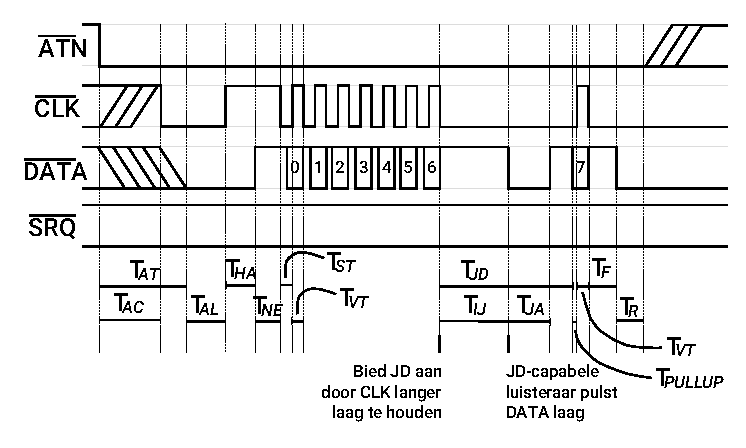
\includegraphics{dutch/images/IEC-Timing-Diagrams/IEC-Timing-Diagram-ATN-JD-Solicit}
\end{center}

\begin{center}
    \setlength{\def\arraystretch{1.5}\tabcolsep}{6pt}
    \small {
    \begin{longtable}{|L{0.6cm}|c|c|c|c|L{6cm}|}
      \hline
        \multicolumn{2}{|c|}{\textbf{Symbool}} & \textbf{Min} & \textbf{4541} & \textbf{Max} & \textbf{Omschrijving} \\
        \hline
        \endhead
        \multicolumn{2}{|c|}{T\textsubscript{JD}} & 320  & 320 & $\infty$ &  Tijd dat CLK op 0V wordt gehouden tussen de twee laatste bits van de byte om het nevenkanaal te markeren; via het nevenkanaal geeft de controller aan dat hij de JiffyDOS{\texttrademark}-protocoluitbeiding wenst te gebruiken.
        \\
        \hline
        \multicolumn{2}{|c|}{T\textsubscript{IJ}} & 100  & -- & 295 &        Tijd voordat de luisteraar de selectie van de JiffyDOS{\texttrademark}-protocoluitbreiding aanvaardt en de bevestiging ervan begint.
        \\
        \hline
        \multicolumn{2}{|c|}{T\textsubscript{IJ}} & 4/100*  & -- & 200 &     Tijd dat de luisteraar de DATA-lijn laag houdt om de selectie van de JiffyDOS{\texttrademark}-protocoluitbreiding te bevestigen.
        \\
        \hline
          \\
\multicolumn{6}{l}{\em Alle tijdseenheden zijn uitgedrukt in microseconden, tenzij anders aangegeven.} \\        \multicolumn{6}{Y{10cm}}{*{}          De 4541 kan pulsbreedtes van slechts 4          microseconden detecteren. Software-implemen\-ta\-ties van het          protocol vereisen echter een grotere waarde. JiffyDOS\texttrademark          gebruikt 100 microseconden.
        }


    \end{longtable}
    }
\end{center}

 \subsection{Verzenden van controller naar apparaat onder JiffyDOS{\texttrademark}}

In tegenstelling tot het standaard seriële protocol maakt het JiffyDOS{\texttrademark}-protocol gebruik van verschillende protocollen voor verzenden en ontvangen. Dit is noodzakelijk bij software-implemen\-ta\-ties om de maximale snelheid te bereiken, omdat de seriële apparaatlijnen op verschillende registerbits zijn gemapt, en een onderdeel van de kracht van het JiffyDOS{\texttrademark}-protocol bestaat uit de slimme manipulatie van de ontvangen bits om het complete byte in de minst mogelijke tijd te reconstrueren, en eveneens bij het verzenden.

Het resultaat is opmerkelijk: JiffyDOS{\texttrademark} kan een byte verzenden in ongeveer dezelfde tijd die het originele protocol nodig heeft om één bit te verzenden!

Let op dat het JiffyDOS{\texttrademark}-protocol databits met de tegenovergestelde polariteit verzendt vergeleken met het standaard protocol: een 1-bit wordt aangegeven met 0V, terwijl een 0-bit wordt aangegeven met 5V.

De SRQ-lijn is niet actief bij deze transactie.

Samengevat:

\begin{enumerate}
 \item Afhankelijk van de toestand van de controller op het moment dat deze met verzenden begint, houdt hij mogelijk de CLK-lijn op 0V. Zo ja, dan laat hij deze onmiddellijk los.\item Vervolgens geeft het apparaat na een willekeurige tijd aan dat het gereed is om een byte van de controller te ontvangen, door de DATA-lijn naar 5V los te laten.\item De timing voor het resterende deel van de byteoverdracht is nu cruciaal, omdat het apparaat direct na het loslaten van DATA de CLK- en DATA-signalen gaat uitlezen om de byte over te dragen.\item De controller wacht enkele microseconden  (T\textsubscript{J6}).\item De controller zet CLK op 0V als databit 4 gelijk is aan 1, en laat deze anders naar 5V los.  De controller zet DATA op 0V als databit 5 gelijk is aan 1, en laat deze anders naar 5V los.\item De controller wacht enkele microseconden  (T\textsubscript{J7}).\item De controller zet CLK op 0V als databit 6 gelijk is aan 1, en laat deze anders naar 5V los.  De controller zet DATA op 0V als databit 7 gelijk is aan 1, en laat deze anders naar 5V los.\item De controller wacht enkele microseconden  (T\textsubscript{J8}).\item De controller zet CLK op 0V als databit 3 gelijk is aan 1, en laat deze anders naar 5V los.  De controller zet DATA op 0V als databit 1 gelijk is aan 1, en laat deze anders naar 5V los.\item De controller wacht enkele microseconden  (T\textsubscript{J9}).\item De controller zet CLK op 0V als databit 2 gelijk is aan 1, en laat deze anders naar 5V los.  De controller zet DATA op 0V als databit 0 gelijk is aan 1, en laat deze anders naar 5V los.\item De controller wacht enkele microseconden  (T\textsubscript{J10}).\item De controller trekt de DATA-lijn naar 0V. Hij laat ook de  CLK-lijn naar 5V los, tenzij hij EOI wil aangeven, in welk  geval hij de CLK-lijn naar 0V trekt.\item De controller wacht enkele microseconden, gedurende welke tijd het  apparaat de EOI-waarde uitleest, en trekt vervolgens DATA naar 0V.  (T\textsubscript{J11}).\item De byteoverdracht is voltooid.
\end{enumerate}

Let er bij het verzenden van de eerste byte onder het JiffyDOS{\texttrademark}protocol op dat het CLK-signaal op 0V kan staan.  De tijd tussen bytes (T\textsubscript{JBB}) is niet vereist (wordt op nul gezet), omdat de korte ontvanglus op het apparaat eenvoudigweg aangeeft wanneer het gereed is om de volgende byte te ontvangen, wat ook bijdraagt aan de hoge snelheid.

Let ook op dat de onderstaande timing gebaseerd is op het moment waarop de signalen ingesteld moeten worden. Bij software-implemen\-ta\-ties moet de latentie van de benodigde processorinstructies in aanmerking worden genomen. Dit vormt geen probleem bij de 4541, omdat deze een latentie van minder dan 50 ns heeft.

\begin{center}
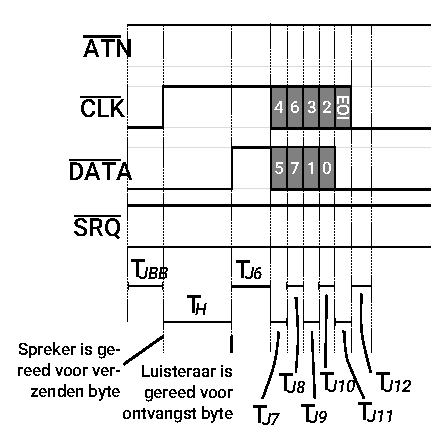
\includegraphics{dutch/images/IEC-Timing-Diagrams/IEC-Timing-Diagram-Send-Byte-JD}
\end{center}

\begin{center}
    \setlength{\def\arraystretch{1.5}\tabcolsep}{6pt}
    \small{
    \begin{longtable}{|L{0.5cm}|c|c|c|c|L{7cm}|}
      \hline
        \multicolumn{2}{|c|}{\textbf{Symbool}} & \textbf{Min} & \textbf{4541} & \textbf{Max} & \textbf{Omschrijving} \\
        \hline
        \endhead
        \multicolumn{2}{|c|}{T\textsubscript{JBB}} & 0  & 0 & $\infty$ &        Tijd tussen bytes.        Er is geen minimale tijd tussen bytes bij het        JiffyDOS{\texttrademark}-protocol,        mits T\textsubscript{J12} voldoende groot is, omdat dat        de latentie van de ontvangroutine effectief verbergt. \\
        \hline
        \multicolumn{2}{|c|}{T\textsubscript{J6}} & 10  & 10 & 10 &        JiffyDOS{\texttrademark} verzenden: insteltijd ontvanger. \\
        \hline
        \multicolumn{2}{|c|}{T\textsubscript{J7}} & 13  & 13 & 13 &        JiffyDOS{\texttrademark} verzenden: vasthoudtijd, eerste di-bit. \\
        \hline
        \multicolumn{2}{|c|}{T\textsubscript{J8}} & 11  & 11 & 11 &        JiffyDOS{\texttrademark} verzenden: vasthoudtijd, tweede di-bit. \\
        \hline
        \multicolumn{2}{|c|}{T\textsubscript{J9}} & 11  & 11 & 11 &        JiffyDOS{\texttrademark} verzenden: vasthoudtijd, derde di-bit. \\
        \hline
        \multicolumn{2}{|c|}{T\textsubscript{J10}} & 12  & 12 & 12 &        JiffyDOS{\texttrademark} verzenden: vasthoudtijd, vierde di-bit. \\
        \hline
        \multicolumn{2}{|c|}{T\textsubscript{J11}} & 15  & 15 & 15 &        JiffyDOS{\texttrademark} verzenden: vasthoudtijd, statusbits. CLK        draagt de EOI-melding, en DATA wordt op 0V gezet om        een succesvolle verzending aan te geven. De ontvanger kan een        framefout aangeven indien DATA 5V wordt waargenomen.  \\
        \hline
        \multicolumn{2}{|c|}{T\textsubscript{J12}} & 18  & 18 & 18 &        JiffyDOS{\texttrademark} hersteltijd na verzending. CLK wordt naar 0V getrokken,        en DATA wordt op 0V gezet om een succesvolle verzending aan te geven.        De ontvanger kan een        framefout aangeven indien DATA 5V wordt waargenomen.  \\
        \hline
        \multicolumn{2}{|c|}{T\textsubscript{JR}} & 15  & 15 & 15 &
        \\
        \hline
        \multicolumn{6}{l}{\em De overige tijden zijn gelijk aan die bij het verzenden van een byte onder Attention.}
          \\
        \multicolumn{6}{l}{\em Alle tijdseenheden zijn uitgedrukt in microseconden, tenzij anders aangegeven.} \\

    \end{longtable}
    }
\end{center}

 \subsection{Ontvangst van randapparaat naar controller onder JiffyDOS{\texttrademark}}

In tegenstelling tot het standaard seriële protocol gebruikt het JiffyDOS{\texttrademark}-protocol verschillende protocollen voor verzenden en ontvangen. Dit is noodzakelijk bij software-implemen\-ta\-ties om de maximale snelheid te bereiken, omdat de seriële randapparatuurbus-lijnen op verschillende registerbits worden gemapt. Een essentieel onderdeel van het JiffyDOS{\texttrademark}-protocol is hoe het op intelligente wijze de ontvangen bits manipuleert om het volledige byte in de kortst mogelijke tijd te reconstrueren, en op vergelijkbare wijze bij verzending.

Het resultaat is opmerkelijk: JiffyDOS{\texttrademark} kan een byte verzenden in ongeveer dezelfde tijd die het originele protocol nodig heeft om één bit te verzenden.

Bij verzending via het JiffyDOS{\texttrademark}-protocol worden de databits geïnverteerd; bij ontvangst van een randapparaat dat het JiffyDOS{\texttrademark}-protocol gebruikt, worden de bits op natuurlijke wijze weergegeven, oftewel met 1 = 5V en 0 = 0V.

De SRQ-lijn is niet actief in deze transactie.

Ter samenvatting:

\begin{enumerate}
\item Het randapparaat kan een willekeurige periode wachten voordat het een byte naar de controller kan verzenden. Wanneer het zover is, laat het de CLK-lijn los naar 5V.\item Wanneer de controller dit opmerkt, laat hij de DATA-lijn los naar 5V en begint het kritieke tijdsgebied van het protocol.\item Het randapparaat wacht kort. Voor apparaten met een software-implemen\-ta\-tie, oftewel alle Commodore{\texttrademark}-stations, is de vertraging een natuurlijk gevolg van de processorinstructie die nodig is om het verzenden van de byte in te luiden; hetzelfde geldt voor de volgende stappen.\item Het randapparaat plaatst het eerste di-bit van gegevens op de CLK- en DATA-lijnen en wacht kort.\item Het randapparaat plaatst het tweede di-bit van gegevens op de CLK- en DATA-lijnen en wacht kort.\item Het randapparaat plaatst het derde di-bit van gegevens op de CLK- en DATA-lijnen en wacht kort.\item Het randapparaat plaatst het vierde di-bit van gegevens op de CLK- en DATA-lijnen en wacht kort.\item Het randapparaat plaatst de statusbits van de byte op de CLK- en DATA-lijnen en wacht kort.\item De controller trekt DATA naar 0V om de ontvangst van de byte te bevestigen en te voorkomen dat het randapparaat nog een byte verzendt voordat hij gereed is.\item Het randapparaat trekt de CLK-lijn naar 0V indien het niet onmiddellijk nog een byte gereed heeft om te verzenden; in het andere geval blijft de lijn op 5V.
\end{enumerate}

De statusbits hebben de volgende betekenis:

\begin{center}
    \setlength{\def\arraystretch{1.5}\tabcolsep}{6pt}
    \begin{longtable}{|c|c|L{7cm}|}
      \hline
        \textbf{CLK} & \textbf{DATA} & \textbf{Betekenis} \\
        \hline
        \endhead
        0V & 0V & Er is een fout opgetreden. \\
        \hline
        0V & 5V & Byte ontvangen met einde-aanduiding (EOI). \\
        \hline
        5V & 0V & Normale byte ontvangen (geen EOI). \\
        \hline
        5V & 5V & Er is een fout opgetreden. \\
        \hline
    \end{longtable}
\end{center}

\begin{center}
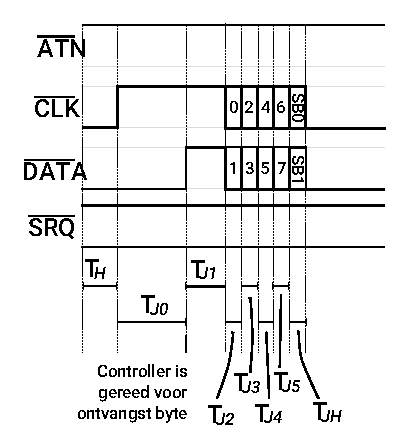
\includegraphics{dutch/images/IEC-Timing-Diagrams/IEC-Timing-Diagram-Receive-Byte-JD}
\end{center}

\begin{center}
    \setlength{\def\arraystretch{1.5}\tabcolsep}{6pt}
    \small{
    \begin{longtable}{|L{0.6cm}|c|c|c|c|L{7cm}|}
      \hline
        \multicolumn{2}{|c|}{\textbf{Symbool}} & \textbf{Min} & \textbf{4541} & \textbf{Max} & \textbf{Omschrijving} \\
        \hline
        \endhead
        \multicolumn{2}{|c|}{T\textsubscript{JH}} & 10  & -- & $\infty$ &        Wachttijd van het randapparaat totdat het gegevens heeft om te verzenden. \\
        \hline
        \multicolumn{2}{|c|}{T\textsubscript{J0}} & 0  & -- & $\infty$ &        Wachttijd van de controller totdat deze gereed is om een byte te ontvangen. \\
        \hline
        \multicolumn{2}{|c|}{T\textsubscript{J1}} & 37  & 37 & $\infty$ &        Deze tijd wordt door soft\-ware-imple\-men\-ta\-ties gebruikt om de byte voor te bereiden voor onmiddellijke verzending. \\
        \hline
        \multicolumn{2}{|c|}{T\textsubscript{J2}} & 14  & 14 & 14 &        Eerste di-bit van gegevens verzenden \\
        \hline
        \multicolumn{2}{|c|}{T\textsubscript{J3}} & 10  & 10 & 10 &        Tweede di-bit van gegevens verzenden \\
        \hline
        \multicolumn{2}{|c|}{T\textsubscript{J4}} & 11  & 11 & 11 &        Derde di-bit van gegevens verzenden \\
        \hline
        \multicolumn{2}{|c|}{T\textsubscript{J5}} & 11  & 11 & 11 &        Vierde di-bit van gegevens verzenden \\
        \hline
        \multicolumn{2}{|c|}{T\textsubscript{JH}} & 13  & 13 & 13 &        Statusbits verzenden \\
        \hline
        \multicolumn{6}{l}{\em De overige tijden zijn gelijk aan die bij het verzenden van een byte onder Attention.}
          \\
        \multicolumn{6}{l}{\em Alle tijdseenheden zijn uitgedrukt in microseconden, tenzij anders aangegeven.} \\

    \end{longtable}
    }
\end{center}



\subsection{Omschakelen van spreker naar luisteraar}

Wanneer de buscontroller een apparaat beveelt om te verzenden, wordt de transactie afgesloten met ATN op 0V. De controller houdt de CLK-lijn op 0V, en het apparaat dat verzond hield de DATA-lijn vast. Deze situatie moet worden omgekeerd: de controller moet de besturing van de bus afstaan en deze overdragen aan het apparaat.

De SRQ-lijn is niet actief bij deze transactie.

Ter samenvatting:

\begin{enumerate}
\item De controller wacht lang genoeg voordat hij de ATN-lijn vrijgeeft, om er zeker van te zijn dat het randapparaat de bevestiging van de byte die onder Attention werd verzonden, heeft afgerond. Dit is de vertraging T\textsubscript{R}.
\item De controller geeft de ATN-lijn vrij naar 5V.
\item De controller wacht enige tijd. Dit is de vertraging T\textsubscript{TK}.
\item De controller geeft de CLK-lijn vrij naar 5V en trekt de DATA-lijn naar 0V. Vanaf dit moment heeft de controller de besturing van de bus afgestaan en wordt hij luisteraar.
\item Na een bepaalde tijdsduur trekt het randapparaat dat op het punt staat te spreken, de CLK-lijn naar 0V en geeft de DATA-lijn vrij, die op 0V blijft staan omdat de controller deze nog steeds naar 0V trekt ter voorbereiding op het ontvangen. Vanaf dit moment is het randapparaat de enige spreker op de bus. De vertraging voordat de CLK-lijn door het randapparaat naar 0V wordt getrokken, is de time-out T\textsubscript{DC}.
\item Het randapparaat wacht enige tijd voordat het met spreken mag beginnen. Dit is de vertraging T\textsubscript{DA}.
\end{enumerate}

Na voltooiing van dit proces zijn de rollen van controller en randapparaat omgekeerd, waarbij het randapparaat nu de rol van spreker (``\textbf{talk}er'') heeft en de controller (en mogelijk andere apparaten op de bus) die van luisteraar (``\textbf{listen}er'').

\begin{center}
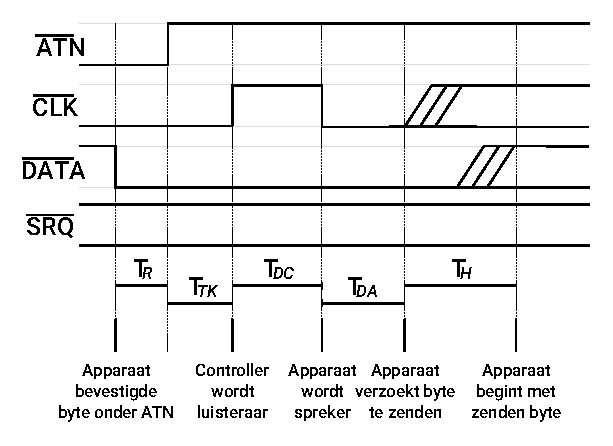
\includegraphics{dutch/images/IEC-Timing-Diagrams/IEC-Timing-Diagram-TurnAround}
\end{center}

\begin{center}
    \setlength{\def\arraystretch{1.5}\tabcolsep}{6pt}
    \small{
    \begin{longtable}{|L{0.6cm}|c|c|c|c|L{6cm}|}
      \hline
        \multicolumn{2}{|c|}{\textbf{Symbool}} & \textbf{Min} & \textbf{4541} & \textbf{Max} & \textbf{Omschrijving} \\
        \hline
        \endhead
        \multicolumn{2}{|c|}{T\textsubscript{DA}} & 4/80* & -- & $\infty$ &        Duur van de bevestiging dat apparaat nu spreker is. De controller houdt CLK.
        \\
        \hline
        \multicolumn{2}{|c|}{T\textsubscript{DC}} & 0 & 64 ms & $\infty$ &        Duur van de zendbevestiging, d.w.z. de tijd die een randapparaat heeft        voordat het spreker wordt. {\em Kan onmiddellijk beginnen zodra CLK op 5V        wordt waargenomen.}\\
        \hline
        \multicolumn{2}{|c|}{T\textsubscript{H}} & -- & N/A & $\infty$ & Luisteraar-wachttijd. {\em De luisteraar kan de ontvangstbevestiging willekeurig lang uitstellen of ook helemaal niet.} \\
        \hline
        \multicolumn{2}{|c|}{T\textsubscript{R}} & 0/20\^{} & 200 & -- & Tijd van        frame tot vrijgave van ATN. \\
        \hline
        \multicolumn{2}{|c|}{T\textsubscript{TK}} & 20 & 40 & 100 & Vrijgave van de        zendvoorwaarde. \\
        \hline
        \multicolumn{6}{l}{\em Alle tijdseenheden zijn uitgedrukt in microseconden, tenzij anders aangegeven.} \\        \multicolumn{6}{Y{10cm}}{* T\textsubscript{DA} wordt geleverd door het randapparaat, niet door de controller. De 4541 is          in staat veel sneller op seriële bus-gebeurtenissen te reageren dan een C64          en heeft derhalve slechts 4 microseconden nodig om te garanderen dat de CLK-lijn          de tijd heeft om naar 5V te stijgen.          Voor controllers met een          softwarematige implementatie van het protocol, zoals de C64,          bedraagt het minimum 80 microseconden.          Randapparaten dienen derhalve steeds          een waarde van ten minste 80 microseconden voor T\textsubscript{DA} te gebruiken.
        } \\
        \multicolumn{6}{Y{10cm}}{\^{} Het          Commodore{\texttrademark} 64 Programmer's Reference Guide          vermeldt          dat T\textsubscript{R} een minimumduur van 20 microseconden heeft.          Wij zien geen aanleiding om te veronderstellen dat          enige implementatie een vertraging vereist          voordat de ATN-lijn kan worden vrijgegeven na het overdragen van          een byte.
        }
          \\
    \end{longtable}
    }
\end{center}

\subsection{Byte verzenden met einde-aanduiding (EOI)}

Na het verzenden van een stroom gegevens wil een apparaat de luisteraar (``\textbf{listen}er'') er vaak van op de hoogte brengen dat het einde van de gegevens is bereikt, bijvoorbeeld zodat deze met de verwerking kan beginnen.  Dit gebeurt door de byte op een bijzondere manier te markeren met het einde-aanduiding (EOI)-attribuut.

Over de betekenis van de afkorting EOI bestaat spraakverwarring. Op de parallele IEE-488 bus heet één van de pinnen in de aansluiting {\em end or identify}. Deze pin heeft inderdaad een dubbele functie: Als ATN niet actief is, dan dient de pin als einde-aanduiding ({\em end}). Is ATN wel actief, dan dient de pin om parallel de status van apparaten op te vragen ({\em identify}). Op de seriële Commodore-bus is de {\em identify}-functie niet aanwezig en is EOI te allen tijde een einde-aanduiding. Wellicht hierom wordt EOI, zelfs in officiële Commodore-documenten, vaak beschreven als {\em end of indicator}.
De meest triviale manier om dit te lezen, "einde van (een) aanduiding", is logisch onzinnig. De juiste manier om dit te lezen is "eind van"-aanduiding, de aanduiding van het eind van gegevensoverdracht. Dit is weer een mooi voorbeeld waarin begrippen in de Engelse taal voor meerdere uitleg vatbaar zijn. We zullen deze spraakverwarring niet meenemen naar het Nederlands en in de handleiding stelselmatig "einde-aanduiding (EOI)" gebruiken.

De einde-aanduiding wordt gerealiseerd met behulp van een timing-nevenkanaal, zodat er geen afzonderlijke ader in de kabel voor nodig is. Wanneer de spreker de CLK-lijn naar 5V heeft gebracht om aan te geven dat hij een byte wil verzenden, en de luisteraar de DATA-lijn naar 5V heeft gebracht om zijn bereidheid om te ontvangen aan te geven, kan de spreker ten minste 200 microseconden wachten om de luisteraar aan te geven dat de byte met EOI-status moet worden ontvangen.  De luisteraar bevestigt dit aan de spreker door de DATA-lijn enige tijd naar 0V te trekken, waarna de verzending vrijwel identiek aan een normale transactie verloopt.

De SRQ-lijn is niet actief bij deze transactie.

Ter samenvatting:

\begin{enumerate}
\item De spreker geeft de CLK-lijn vrij naar 5V om aan te geven dat hij een byte wil verzenden.
\item Na een willekeurige tijdsduur geeft de luisteraar de DATA-lijn vrij naar 5V om zijn bereidheid om een byte te ontvangen aan te geven.
\item Normaal zou de spreker op dit punt na een korte tijd beginnen met het verzenden van de bits.  Om EOI aan te geven, wacht hij evenwel stilzwijgend totdat de luisteraar doorheeft dat deze byte afwijkend is, hetgeen ertoe leidt dat de luisteraar de DATA-lijn terug naar 0V trekt.
\item De luisteraar houdt de DATA-lijn lang genoeg op 0V om er zeker van te zijn dat de spreker dit heeft opgemerkt, en geeft deze vervolgens weer vrij.
\item Zodra de spreker heeft waargenomen dat de luisteraar de DATA-lijn naar 0V heeft getrokken en weer heeft vrijgegeven, begint hij de byte na een korte vertraging normaal te verzenden.
\item Indien de spreker te lang wacht, neemt de luisteraar aan dat de spreker EOI wilde aangeven zonder daadwerkelijk een byte te verzenden.  \item De verzending van de byte wordt op dezelfde manier afgerond als bij een niet-EOI-byte.
\end{enumerate}


\begin{center}
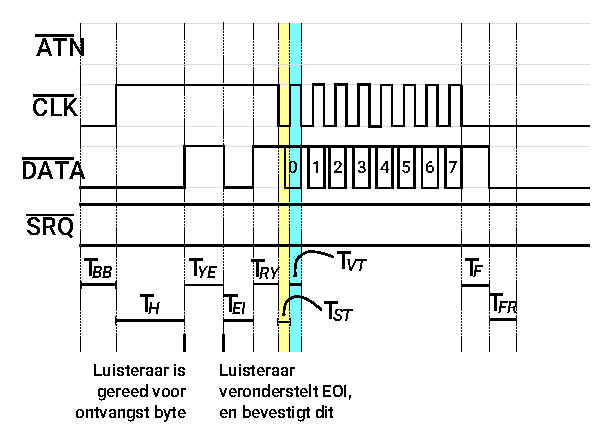
\includegraphics{dutch/images/IEC-Timing-Diagrams/IEC-Timing-Diagram-Send-Byte-EOI}
\end{center}

\begin{center}
    \setlength{\def\arraystretch{1.5}\tabcolsep}{6pt}
    \small{
    \begin{longtable}{|L{0.6cm}|c|c|c|c|L{6cm}|}
      \hline
        \multicolumn{2}{|c|}{\textbf{Symbool}} & \textbf{Min} & \textbf{4541} & \textbf{Max} & \textbf{Omschrijving} \\
        \hline
        \endhead
        \multicolumn{2}{|c|}{T\textsubscript{BB}} & 100 & 100 & $\infty$ &        Tijd tussen bytes. Sprekers moeten lang genoeg wachten om de luisteraar de tijd te geven het einde van de verzending van        de vorige byte te registreren, voordat de volgende byte kan worden verzonden. \\
        \hline
        \multicolumn{2}{|c|}{T\textsubscript{H}} & -- & N/A & $\infty$ & Luisteraar-wachttijd. {\em De luisteraar kan de ontvangstbevestiging willekeurig lang uitstellen of ook helemaal niet.} \\
        \hline
         \multicolumn{2}{|c|}{T\textsubscript{YE}} & 200 & 250 & $\infty$ &        EOI-indicatievertraging. De zender moet ten minste 200        microseconden wachten zodat de ontvanger kan herkennen dat een byte        met EOI wordt verzonden. Indien de vertraging korter is,        herkent de ontvanger de EOI niet. \\
        \hline
         \multicolumn{2}{|c|}{T\textsubscript{EI}} & 60 & 80 & $\infty$ &        EOI-bevestiging vasthoudtijd. De ontvanger moet de DATA-lijn ten minste 60 microseconden weer op 0V trekken, zodat de        zender deze EOI-bevestigingspuls kan detecteren. \\
        \hline
         \multicolumn{2}{|c|}{T\textsubscript{RY}} & 60 & 80 & 100 &        De spreker dient binnen een strak tijdvenster te reageren. Indien hij te vroeg is, is het mogelijk dat de luisteraar zich na bevestiging van de EOI, nog niet heeft voorbereid op ontvangst en kan de synchronisatie verloren gaan. Indien hij te laat is, dan kan de luisteraar concluderen dat de spreker gestopt is met spreken. \\
        \hline
         \multicolumn{2}{|c|}{T\textsubscript{ST}} & 20*  & 35 & $\infty$ &        Databit-insteltijd. {\em In de C64 Programmer's Reference Guide          aangeduid als T\textsubscript{S}.}\\
        \hline
         \multicolumn{2}{|c|}{T\textsubscript{VT}} & 20*  & 35 & $\infty$ &        Databit-geldigheidsvasthoudtijd. {\em In de C64 Programmer's          Reference Guide aangeduid als          T\textsubscript{V}.} \\
        \hline
         \multicolumn{2}{|c|}{T\textsubscript{F}} & --  & 1000 & 1000 &        Frame-handshake (bevestiging) time-out. \\
        \hline
         \multicolumn{2}{|c|}{T\textsubscript{FR}} & 0/60\^ & 0 & $\infty$ &        EOI-frame-bevestiging. De luisteraar trekt DATA na een        korte periode naar 0V om de met EOI verzonden byte te bevestigen. \\
        \hline
         \multicolumn{6}{l}{\em Alle tijdseenheden zijn uitgedrukt in microseconden, tenzij anders aangegeven.} \\        \multicolumn{6}{Y{10cm}}{* T\textsubscript{ST} wordt          geleverd door het randapparaat, niet door de controller. De 4541 is          in staat veel sneller te reageren op seriële bus-gebeurtenissen dan een C64,          en heeft derhalve slechts 4 microseconden nodig om er zeker van te zijn dat          de CLK-lijn de tijd heeft gehad naar 5V te stijgen.          Voor controllers die een softwarematige implementatie          van het protocol gebruiken, zoals de C64,          bedraagt het minimum 80 microseconden.          Randapparaten dienen derhalve altijd een          waarde van ten minste 80 microseconden voor T\textsubscript{DA}          te gebruiken.
        } \\
         \multicolumn{6}{Y{10cm}}{\^{} De          Commodore{\texttrademark} 64 Programmer's Reference Guide          vermeldt          T\textsubscript{FR} met een minimumduur van 60 microseconden.          Wij zien geen enkel bewijs          dat er een vertraging nodig zou zijn          voordat de DATA-lijn door de luisteraar laag kan worden getrokken          om ontvangst van een byte te bevestigen.
        }
          \\
    \end{longtable}
    }
\end{center}

 \subsection{Byte ontvangen}

 Het ontvangen van bytes op de IEC-bus verloopt identiek aan het verzenden.        Het belangrijkste verschil is dat de 4541 veel ruimere        marginale waarden voor tijdsparameters toelaat dan softwarematige implementaties van het bus-protocol. De 4541 heeft niet meer dan 4 microseconden nodig voor een        willekeurige bus-toestand; dit is de tijd die de pull-up-weerstanden        op de bus nodig hebben om de lijnen te laten terugkeren naar 5V.        Intern is de 4541 in staat bit-tijden korter dan 1 microseconde te detecteren.

 \section{Optionele geïntegreerde datalogger}

 De 4541 is verkrijgbaar in een variant die een ingebouwde seriële        randapparatuurbus-datalogger bevat. Deze is ontworpen om het oplossen van        protocolfouten op deze bus te vergemakkelijken. Het vastleggen van gegevens begint zodra        opdracht \$D0 aan de 4541 wordt gegeven, en        duurt ongeveer 4 milliseconden.

\begin{itemize}
   \item {\bf DATALOG0} Het lage byte van de optionele geïntegreerde seriële    randapparatuurbus-datalogger. Het schrijven van \$00 naar dit register    reset het leespunt van de datalogger naar het begin van de    opname. Het schrijven van \$01 naar dit register    verplaatst het leespunt van de datalogger met één tijdstap.    De tijdstappen bedragen ongeveer 1 microseconde, met extra        tijdstappen wanneer een van de signalen op de seriële        perifere bus van toestand verandert.    \item {\bf DATALOG1} Het hoge byte van de optionele geïntegreerde seriële      randapparatuurbus-datalogger. Verschillende velden kunnen op dit      adres worden gelezen door de volgende waarden naar het DATALOG0-register te schrijven:
      \begin{itemize}
         \item \$02 - Lees lage byte van het statemachine-toestandsnummer van de IEC-controller.        \item \$03 - Lees hoge byte van het statemachine-toestandsnummer van de IEC-controller.        \item \$04 - Lees lage byte van het aantal cycli dat de vorige bustoestand        is vastgehouden.        \item \$05 - Lees hoge byte van het aantal cycli dat de vorige bustoestand        is vastgehouden.
        \end{itemize}
\end{itemize}

 Elke tijdstap legt 16 bits informatie vast over de seriële        perifere bus:
\begin{itemize}
 \item {\bf DATALOG0 Bit 0} DATA-lijn invoerwaarde\item {\bf DATALOG0 Bit 1} CLK-lijn invoerwaarde\item {\bf DATALOG0 Bit 2} SRQ-lijn invoerwaarde\item {\bf DATALOG0 Bit 3} DATA-lijn uitvoertoestand\item {\bf DATALOG0 Bit 4} CLK-lijn uitvoertoestand\item {\bf DATALOG0 Bit 5} SRQ-lijn uitvoertoestand\item {\bf DATALOG0 Bit 6} ATN-lijn uitvoertoestand\item {\bf DATALOG0 Bit 7} RESET-lijn uitvoertoestand\item {\bf DATALOG1} Toegang tot de aanvullende datalogger-velden.
\end{itemize}

 De invoerwaarden zijn de spanningen die de 4541 op de        betreffende pinnen uitleest. Los daarvan legt de datalogger vast of de 4541        een van die lijnen laag trekt. Dit maakt het mogelijk te bepalen of        een aangesloten randapparaat of de 4541 een bepaald signaal laag        trekt. Dit biedt veel meer informatie dan het simpelweg signalen        op de seriële randapparatuurbus meten, waarbij niet eenvoudig is vast te stellen wie        een bepaalde lijn laag trekt.

 De volgende waarheidstabel legt uit hoe deze signalen moeten worden geïnterpreteerd:

\begin{center}
    \setlength{\def\arraystretch{1.5}\tabcolsep}{6pt}
    \small{
    \begin{longtable}{|c|c|L{8cm}|}
        \hline
         \textbf{Invoerwaarde} & \textbf{Uitvoerwaarde} &        \textbf{Betekenis}  \\
        \hline
        \endhead
         1 & 1 & Het signaal zweeft op 5V. Geen enkel apparaat trekt het laag. \\
        \hline
         0 & 1 & Het signaal staat op 0V. De 4541 trekt het niet laag, ofwel een aangesloten randapparaat, ofwel de CIA trekt het laag. \\
        \hline
         0 & 0 & Het signaal staat op 0V. De 4541 trekt het laag. Andere apparaten kunnen het ook laag trekken, maar tussen deze twee situaties kan niet worden onderscheiden. \\
        \hline
         1 & 0 & Het signaal zweeft op 5V, maar de 4541 trekt het naar 0V. Uw computer is waarschijnlijk defect, of iemand heeft 5V op het signaal aangesloten zonder stroombeperkende        weerstand ertussen; in dat geval is uw computer op het punt defect te raken. \\
        \hline
    \end{longtable}
    }
\end{center}

\subsection{Gegevens uit de datalogger halen}

Met het volgende programma wordt de inhoud van de datalogger opgehaald en als PETSCII-golfvorm weergegeven, zoals de hier getoonde:

\begin{center}
  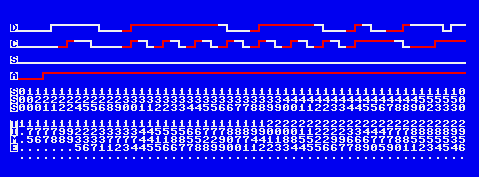
\includegraphics[width=0.7\linewidth]{images/IEC-Timing-Diagrams/iec-waveform-cropped}
\end{center}


% Program is too long to fit on a single page
\input{examples/iec-data-logger}
\input{examples/iec-data-logger-2}
